\setcounter{section}{0}
\setcounter{viduii}{0}
	\viduii{3}{	Hai xe chuyển động đều trên cùng một đường thẳng. Vận tốc của xe (I) là $\SI{20}{\meter/\second}$, xe (II) là $\SI{10}{\meter/\second}$. Lúc $t=0$, hai xe cách nhau $\SI{200}{\meter}$. Chọn gốc tọa độ là vị trí của xe (I) lúc $t=0$, chiều dương là chiều chuyển động của hai xe.
	\begin{enumerate}[label=\alph*)]
		\item Viết phương trình chuyển động của mỗi xe.
		\item Vẽ đồ thị chuyển động của hai xe, từ đồ thị hãy xác định thời điểm và nơi gặp nhau của hai xe.
	\end{enumerate}
}
{	\begin{center}
		\textbf{Hướng dẫn giải}
	\end{center}
	
	
	\begin{enumerate}[label=\alph*)]
		\item
		Hệ quy chiếu gồm:
		\begin{itemize}
			\item Chiều dương là chiều chuyển động của hai xe;
			\item Gốc tọa độ là vị trí của xe (I) lúc $t=0$;
			\item Mốc thời gian ($t=0$) là lúc hai xe cách nhau $\SI{200}{\meter}$.
		\end{itemize}
		
		Phương trình chuyển động của vật (I) là:
		\begin{equation*}
			x_\text{(I)}=x_{0\text{(I)}} + v_\text{(I)}t =20t\textrm{ (m, s)}.
		\end{equation*}
		
		Phương trình chuyển động của vật (II) là:
		\begin{equation*}
			x_\text{(II)}=x_{0\text{(II)}} + v_\text{(II)}t = 200+10t\textrm{ (m, s)}.
		\end{equation*}
		\item
		Đồ thị chuyển động của hai xe là:
		\begin{center}
			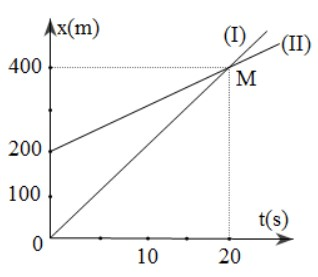
\includegraphics[scale=0.8]{../figs/VN10-PH-03-L-002-4-V2-02.jpg}
		\end{center}
		Hai đồ thị cắt nhau tại M ($t_M=\SI{20}{\second}$, $x_M=\SI{400}{\meter}$). Do đó, nơi gặp cách vị trí xe (I) lúc $t=0$ là $\SI{400}{\meter}$ sau thời gian $\SI{20}{\second}$.
	\end{enumerate}	
}
	\viduii{3}{Hai bến sông A  và B cách nhau 11,2 km. Một chiếc ca nô phải mất bao nhiêu thời gian để đi từ A đến B rồi trở lại ngay từ B về A? Biết vận tốc của ca nô so với nước không chảy là $v_1=$ 15 km/h và vận tốc của nước với bờ sông là $v_2=$ 1 km/h.
	
}
{	\begin{center}
		\textbf{Hướng dẫn giải}
	\end{center}
	
	Ta gọi $v_{\text{xd}}, v_{\text{nd}}$ lần lượt là vận tốc của thuyền khi nó xuôi dòng và ngược dòng.
	
	Vận tốc của thuyền đối với bờ khi thuyền đi xuôi dòng là:
	$$v_{\text{xd}}=v_1+v_2 = 16\,\textrm{km/h}.$$
	Thời gian thuyền đi xuôi dòng khi nó đi từ A đến B:
	$$t_{\text{xd}}=\dfrac{AB}{v_{\text{xd}}}=\text{0,7} \,\text{h}.$$
	Vận tốc của thuyền đối với bờ khi thuyền đi ngược dòng là:
	$$v_{\text{nd}}=v_1-v_2 = 14\,\textrm{km/h}.$$
	Thời gian thuyền đi ngược dòng khi nó đi từ B đến A:
	$$t_{\text{nd}}=\dfrac{AB}{v_{\text{nd}}}=\text{0,8}\, \text{h}.$$
	Thời gian ca nô đi từ A đến B và từ B về A là:
	
	$$t= t_{\text{xd}}+ t_{\text{nd}}=\text{1,5}\,\text{h}.$$
}

\begin{enumerate}[label=\bfseries Câu \arabic*:]
	\item \mkstar{2}
	
	{
		Hãy vẽ đồ thị độ dịch chuyển - thời gian trong chuyển động của A theo bảng ghi số liệu vào vở. Trên trục tung (trục độ dịch chuyển) $\SI{1}{cm}$ ứng với $\SI{200}{m}$; trên trục hoành (trục thời gian) $\SI{1}{cm}$ ứng với $\SI{50}{s}$.
		
		\begin{center}
			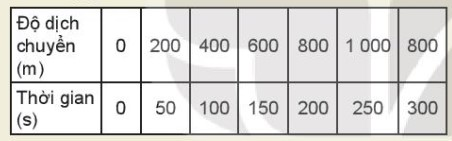
\includegraphics[scale=1]{../figs/VN10-2022-PH-TP006-5.jpg}
		\end{center}
		
	}
	\hideall{
		
	Từ bảng số liệu ta vẽ được đồ thị như hình sau:
	
	
		\begin{center}
			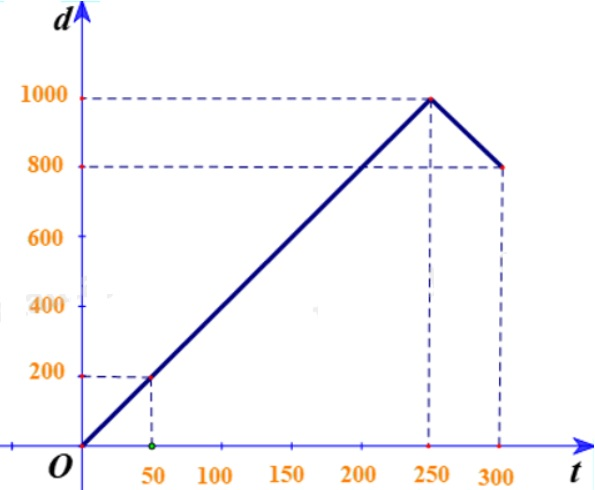
\includegraphics[scale=0.6]{../figs/VN10-2022-PH-TP006-6.jpg}
		\end{center}
	
	}

	\item \mkstar{3}
	
	{
		Hãy tính quãng đường đi được, độ dịch chuyển, tốc độ, vận tốc của bạn A khi đi từ nhà đến trường và khi đi từ trường đến siêu thị. Coi chuyển động của bạn A là chuyển động đều và biết cứ $\SI{100}{m}$ bạn A đi hết $\SI{25}{s}$.
		\begin{center}
			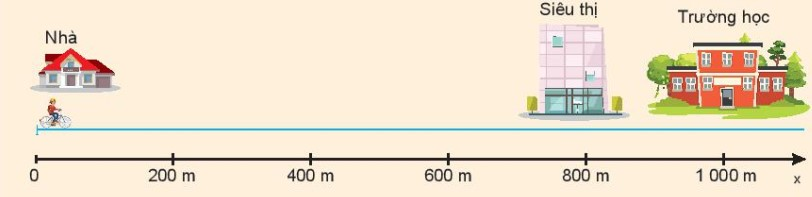
\includegraphics[scale=0.9]{../figs/VN10-2022-PH-TP006-1.jpg}
		\end{center}
	}
	
	\hideall{
		
	Vì bạn A đi từ nhà đến trường là theo 1 hướng, không đổi hướng nên :
	
	Quãng đường đi được và độ dịch chuyển là như nhau và bằng $\SI{1000}{m}$.
	
	Vận tốc và tốc độ là như nhau và bằng : 
	
	$$v = \dfrac{d}{t} =\dfrac{100}{25} = \SI{4}{m/s}.$$
	}
	
		\item \mkstar{3}
	
	{
		Đồ thị độ dịch chuyển - thời gian của một người đang bơi trong một bể bơi dài $\SI{50}{m}$. 
		\begin{center}
			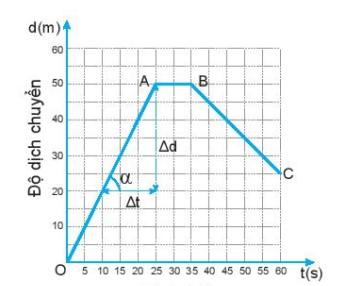
\includegraphics[scale=1]{../figs/VN10-2022-PH-TP006-2.jpg}
		\end{center}
	}
		Trong 25 giây đầu mỗi giây người đó bơi được bao nhiêu mét? Tính vận tốc của người đó ra m/s. Từ giây nào đến giây nào người đó không bơi?
	\hideall{
		
		Từ đồ thị ta thấy, trong 25 giây đầu người đó chuyển động thẳng từ O – A và không đổi chiều, độ dịch chuyển trong 25 giây đầu là $\SI{50}{m}$.
		
		Mỗi giây người đó bơi được:
		
		$$\dfrac{50}{25} = \SI{2}{m}.$$
		
		Vận tốc của người đó:
		
		$$v = \dfrac{d}{t} = \dfrac{50}{25} = \SI{2}{m/s}.$$
		
		Từ A – B: người đó không bơi $\Rightarrow$ Người đó không bơi từ giây 25 đến giây 35.
	
	}
		\item \mkstar{3}
	
	{
		Đồ thị độ dịch chuyển - thời gian của một người đang bơi trong một bể bơi dài $\SI{50}{m}$. 
		\begin{center}
			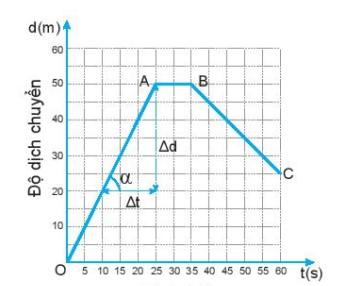
\includegraphics[scale=1]{../figs/VN10-2022-PH-TP006-2.jpg}
		\end{center}
	}
	Từ giây 35 đến giây 60 người đó bơi theo chiều nào? Trong 20 giây cuối cùng, mỗi giây người đó bơi được bao nhiêu mét? Tính vận tốc của người đó ra m/s.
	\hideall{
		
		Từ giây 35 đến giây 60 người đó bơi ngược chiều dương.
		
		Trong 20 giây cuối cùng:
		
		Từ đồ thị ta thấy
		
		- Giây thứ 40 có $d_1 = \SI{45}{m}$.
		
		- Giây thứ 60 có $d_2 =  \SI{25}{m}$.
		
		$\Rightarrow$ Trong 20 giây cuối, mỗi giây người đó bơi được 
		
		$$\dfrac{|25 - 15|}{20} = \SI{1}{m}.$$
		
		- Vận tốc của người đó là
		
		$$v = \dfrac{\Delta d}{\Delta t} = \dfrac{d_2 - d_1}{\Delta t} = -\SI{1}{m/s}.$$
		
		
		
	}
		\item \mkstar{3}
	
	{
		Đồ thị độ dịch chuyển - thời gian của một người đang bơi trong một bể bơi dài $\SI{50}{m}$. 
		\begin{center}
			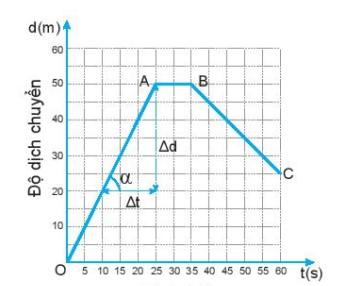
\includegraphics[scale=1]{../figs/VN10-2022-PH-TP006-2.jpg}
		\end{center}
	}
	Xác định độ dịch chuyển và vận tốc của người đó khi bơi từ B đến C.
	\hideall{
		
		- Tại B: $d_1 = \SI{50}{m}; t_1 = \SI{35}{s}.$
		
		- Tại C: $d_2 = \SI{25}{m}; t_2 = \SI{60}{s}.$
		
		Từ B đến C, độ dịch chuyển là
		
		$$\Delta d = d_2 - d_1 = - \SI{25}{m}.$$
		
		Vận tốc của người đó khi bơi từ B đến C l
		
		$$ v = \dfrac{\Delta d}{\Delta t} = - \SI{1}{m/s}.$$
		
	}
		\item \mkstar{3}
	
	{
		Đồ thị độ dịch chuyển - thời gian của một người đang bơi trong một bể bơi dài $\SI{50}{m}$. 
		\begin{center}
			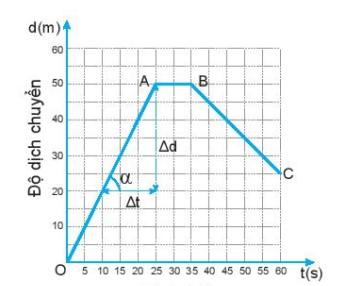
\includegraphics[scale=1]{../figs/VN10-2022-PH-TP006-2.jpg}
		\end{center}
	}
	Xác định độ dịch chuyển và vận tốc của người đó trong cả quá trình bơi.
	\hideall{
		
		Độ dịch chuyển của người đó trong cả quá trình bơi là
		
		$$\Delta d = \SI{25}{m}.$$
		
		Vận tốc của người đó trong cả quá trình bơi là
		
		$$v = \dfrac{\Delta d}{\Delta t} \approx \SI{0,417}{m/s}.$$
		
		

	
	}
		\item \mkstar{3}
	
	{
		Đồ thị độ dịch chuyển - thời gian của một người đang bơi trong một bể bơi dài $\SI{50}{m}$. 
		\begin{center}
			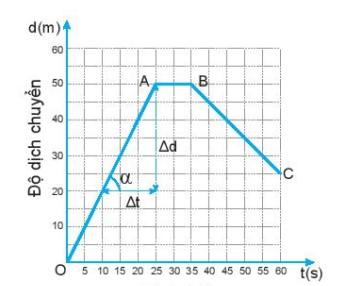
\includegraphics[scale=1]{../figs/VN10-2022-PH-TP006-2.jpg}
		\end{center}
	}
	Hãy xác định vận tốc và tốc độ của người bơi từ giây 45 đến giây 60.
	\hideall{
		
		Độ dịch chuyển:
		
		$$d = 40 - 25 = \SI{15}{m}.$$
		
		Vận tốc là:
		
		$$v = \dfrac{d}{t} = \dfrac{15}{15} = \SI{1}{m/s}.$$
		
		Vì từ giây thứ 45 đến 60, người bơi bơi theo cùng 1 hướng không đổi nên tốc độ bằng vận tốc và bằng $\SI{1}{m/s}$.
	}
		\item \mkstar{3}
	
	{
		Số liệu về độ dịch chuyển và thời gian của chuyển động thẳng của một xe ô tô đồ chơi chạy bằng pin được ghi trong bảng bên: 
		\begin{center}
			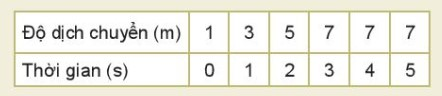
\includegraphics[scale=1]{../figs/VN10-2022-PH-TP006-3.jpg}
		\end{center}
	
		Dựa vào bảng để:
	
	\begin{enumerate}[label=\alph*)]
		\item Vẽ đồ thị độ dịch chuyển - thời gian của chuyển động.
		\item Mô tả chuyển động của xe.
		\item Tính vận tốc của xe trong $\SI{3}{s}$ đầu.
	\end{enumerate}
		}
	\hideall{
		
		\begin{enumerate}[label=\alph*)]
			\item Vẽ đồ thị độ dịch chuyển - thời gian của chuyển động
			
			\begin{center}
				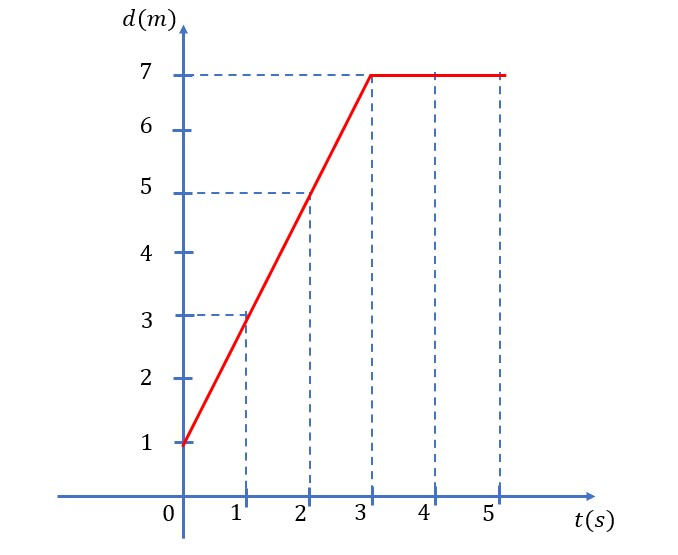
\includegraphics[scale=0.6]{../figs/VN10-2022-PH-TP006-7.jpg}
			\end{center}
			
			\item Mô tả chuyển động của xe
			
			- Từ 0 – 3 giây: xe chuyển động thẳng.
			
			- Từ giây thứ 3 đến giây thứ 5: xe đứng yên (dừng lại).
			
			
			\item 
			Độ dịch chuyển của xe trong 3 giây đầu là:
			
			$$d = 7-1 = \SI{6}{m}.$$
			
			Vận tốc của xe trong $\SI{3}{s}$ đầu
			
			$$v = \dfrac{\Delta d}{\Delta t} = \SI{2}{m/s}.$$
			
		\end{enumerate}
	}
		\item \mkstar{3}
	
	{
		Đồ thị độ dịch chuyển - thời gian trong chuyển động thẳng của một xe ô tô đồ chơi điều khiển từ xa được vẽ ở hình: 
		\begin{center}
			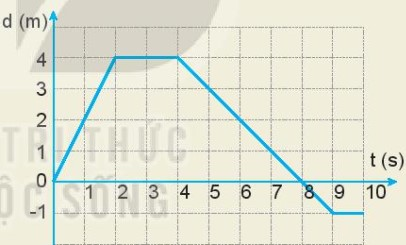
\includegraphics[scale=1]{../figs/VN10-2022-PH-TP006-4.jpg}
		\end{center}
		
		
		\begin{enumerate}[label=\alph*)]
			\item Mô tả chuyển động của xe.
			\item Xác định vị trí của xe so với điểm xuất phát của xe ở giây thứ 2, giây thứ 4, giây thứ 8 và giây thứ 10.
		\end{enumerate}
	}
	\hideall{
		
		\begin{enumerate}[label=\alph*)]
			\item Mô tả chuyển động của xe
			
			- Trong 2 giây đầu: xe chuyển động thẳng
			
			- Từ giây thứ 2 đến giây thứ 4: xe đứng yên
			
			- Từ giây thứ 4 đến giây thứ 10: xe chuyển động thẳng theo chiều ngược lại.
			
			- Từ giây thứ 9 đến giây thứ 10: xe dừng lại.
	
			\item 
			
			- Ở giây thứ 2: xe ở vị trí cách điểm xuất phát $\SI{4}{m}$.
			
			- Ở giây thứ 4: xe ở vị trí cách điểm xuất phát $\SI{4}{m}$.
			
			- Ở giây thứ 8: xe trở về vị trí xuất phát.
			
			- Ở giây thứ 10: xe ở vị trí cách điểm xuất phát $\SI{1}{m}$ theo chiều âm.
			
		\end{enumerate}
	}
		\item \mkstar{3}
	
	{
		Đồ thị độ dịch chuyển - thời gian trong chuyển động thẳng của một xe ô tô đồ chơi điều khiển từ xa được vẽ ở hình: 
		\begin{center}
			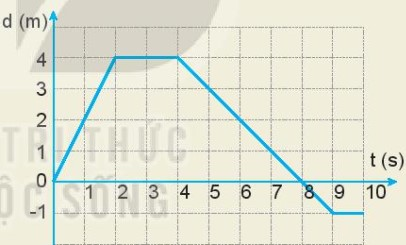
\includegraphics[scale=1]{../figs/VN10-2022-PH-TP006-4.jpg}
		\end{center}
		
		
		\begin{enumerate}[label=\alph*)]
			\item Xác định tốc độ và vận tốc của xe trong 2 giây đầu, từ giây 2 đến giây 4 và từ giây 4 đến giây 8.
			\item Xác định quãng đường đi được và độ dịch chuyển của xe sau 10 giây chuyển động. Tại sao giá trị của chúng không giống nhau?
		\end{enumerate}
	}
	\hideall{
		
		\begin{enumerate}[label=\alph*)]
			\item Xác định tốc độ và vận tốc của xe
			
			- Trong 2 giây đầu, xe chuyển động thẳng, không đổi chiều nên tốc độ bằng vận tốc:
			
			$$v = \dfrac{d}{t} = \SI{2}{m/s}.$$
			
			- Từ giây 2 đến giây 4: xe đứng yên nên vận tốc và tốc độ của xe đều bằng 0.
			
			- Từ giây 4 đến giây 8:
			
			+ Tốc độ:
			
			$$v = \dfrac{s}{t} = \SI{1}{m/s}.$$
			
			+ Vận tốc:
			
			$$v = \dfrac{\Delta d}{\Delta t} = -\SI{1}{m/s}.$$
			

			\item
			- Từ đồ thị, ta thấy quãng đường đi được của xe sau 10 giây chuyển động là:
			
			$$s = 4 + 4 + 1 = \SI{9}{m}.$$
			
			- Độ dịch chuyển của xe sau 10 giây là:
			
			$$d = - 1 - 4 + 4 = - \SI{1}{m}.$$
			
			Suy ra quãng đường và độ dịch chuyển của xe sau 10 giây không giống nhau vì xe chuyển động theo 2 chiều.
			
		\end{enumerate}
		
	}
			\item \mkstar{3}

{Một ô tô A chạy đều trên một đường thẳng với vận tốc $\SI{40}{km/h}$. Một ô tô B đuổi theo ô tô A với vận tốc $\SI{60}{km/h}$. Xác định vận tốc của ô tô B đối với ô tô A và của ô tô A đối với ô tô B.}
\hideall{
	Chọn chiều dương là chiều chuyển động của hai xe.
	
	$\overrightarrow{v_\text{AD}}$ là vận tốc của xe A đối với đất;
	
	$\overrightarrow{v_\text{BD}}$ là vận tốc của xe B đối với đất;
	
	$\overrightarrow{v_\text{BA}}$ là vận tốc của xe B đối với xe A.
	
	Theo công thức cộng vận tốc:
	$$\overrightarrow{v_\text{AB}} = \overrightarrow{v_\text{AD}}+\overrightarrow{v_\text{DB}} \Rightarrow \overrightarrow{v_\text{AB}} = \overrightarrow{v_\text{AD}} - \overrightarrow{v_\text{BD}}$$
	
	Do hai xe chuyển động ngược chiều nên
	$$v_\text{AB} = 40-60=-20\ \text{km/h}$$
	
	Vậy $v_\text{BA} = 20\ \text{km/h}$.
}
\item \mkstar{3}


{A ngồi trên một toa tàu chuyển động với vận tốc $\SI{15}{km/h}$ đang rời ga. B ngồi trên một toa tàu khác đang chuyển động với vận tốc $\SI{10}{km/h}$ đang đi ngược chiều vào ga. Hai đường tàu song song với nhau. Tính vận tốc của B đối với A.
}
\hideall
{Chọn chiều dương là chiều chuyển động của tàu A.
	
	$\overrightarrow{v_\text{AD}}$ là vận tốc của tàu A đối với đất;
	
	$\overrightarrow{v_\text{BD}}$ là vận tốc của tàu B đối với đất;
	
	$\overrightarrow{v_\text{BA}}$ là vận tốc của tàu B đối với tàu A.
	
	Theo công thức cộng vận tốc:
	$$\overrightarrow{v_\text{BD}} = \overrightarrow{v_\text{BA}}+\overrightarrow{v_\text{AD}} \Rightarrow \overrightarrow{v_\text{BA}} = \overrightarrow{v_\text{BD}} - \overrightarrow{v_\text{AD}}=\overrightarrow{v_\text{BD}} + \overrightarrow{-v_\text{AD}}$$
	
	Do A và B chuyển động ngược chiều nên
	$$v_\text{AB} = v_\text{BD} + v_\text{DA} = -10-15 = \SI{-25}{km/h}$$
	
	Vận tốc của tàu B đối với tàu A có độ lớn $\SI{25}{km/h}$ và ngược chiều so với chiều chuyển động của tàu A.
}
\item \mkstar{3}


{
	Hai người đi xe đạp từ A đến C, người thứ nhất đi theo đường từ A đến B, rồi từ B đến C; người thứ hai đi thẳng từ A đến C. Cả hai đều về đích cùng một lúc. Hãy tính quãng đường đi được và độ dịch chuyển của người thứ nhất và người thứ hai. So sánh và nhận xét kết quả.
	
	\begin{center}
		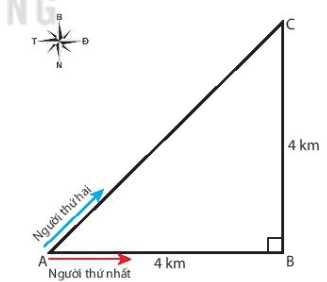
\includegraphics[scale=1]{../figs/VN10-2022-PH-TP004-5.jpg}
	\end{center}
}

\hideall
{	
	
	Quãng đường đi được của người thứ nhất:
	
	$$s_1 = \text{AB} + \text{BC} = 4+4 = \SI{8}{km}.$$
	
	Vì ABC là tam giác vuông nên độ lớn của độ dịch chuyển $\vec{\text{AC}}$ của người thứ nhất được tính bằng công thức:
	
	$$d_1 = \sqrt{\text{AB}^2 + \text{BC}^2} \approx \SI{5,7}{km}.$$
	
	Vì ABC là tam giác vuông cân nên góc CAB bằng $45^\circ$. Hướng của độ dịch chuyển là hướng $45^\circ$ Đông - Bắc. Độ dịch chuyển của người thứ nhất là $d_1 = \SI{5,7}{km}$ (hướng $45^\circ$ Đông - Bắc).
	
	Quãng đường đi được của người thứ hai là:
	
	$$s_2 = \text{AC} = \SI{5,7}{km}.$$
	
	Độ dịch chuyển của người thứ hai là:
	
	$$d_2 = \SI{5,7}{km}$$
	
	và hướng $45^\circ$ Đông - Bắc.
}

\item \mkstar{3}


{   
	Trên đoàn tàu đang chạy thẳng với vận tốc trung bình $\SI{36}{km/h}$ so với mặt đường. Hãy xác định vận tốc của hành khách đối với mặt đường nếu người này chuyển động về cuối đoàn tàu với vận tốc có cùng độ lớn $\SI{1}{m/s}$.
}
\hideall
{
	
	Đổi: $\SI{36}{km/h} = \SI{10}{m/s}$.
	
	Gọi:
	
	$\vec v_{1,2}$ là vận tốc của hành khách so với tàu.
	
	$\vec v_{2,3}$ là vận tốc của tàu so với mặt đường.
	
	$\vec v_{1,3}$ là vận tốc của hành khách so với mặt đường.
	
	Ta có:
	
	$$\vec v_{1,3} = \vec v_{1,2} + \vec v_{2,3}.$$
	
	Do hành khách chuyển động về cuối đoàn tàu, tức là ngược chiều chuyển động của đoàn tàu nên ta có:
	
	$$v_{1,3} = - v_{1,2} + v_{2,3} = \SI{9}{m/s}.$$
	
	
}
\item \mkstar{3}


{
	Một người bơi trong bể bơi yên lặng có thể đạt tới vận tốc $\SI{1}{m/s}$. Nếu người này bơi xuôi dòng sông có dòng chảy với vận tốc $\SI{1}{m/s}$ thì có thể đạt vận tốc tối đa là bao nhiêu?
}
\hideall
{
	Gọi:
	
	$\vec v_{1,2}$ là vận tốc của người so với nước.
	
	$\vec v_{2,3}$ là vận tốc của nước so với bờ.
	
	$\vec v_{1,3}$ là vận tốc của người so với bờ.
	
	Ta có:
	
	$$\vec v_{1,3} = \vec v_{1,2} + \vec v_{2,3}.$$
	
	- Khi người bơi trong bể nước yên lặng, thì $v_{2,3} = 0$:
	
	$$v_{1,2} = v_{1,3} = \SI{1}{m/s}.$$
	
	- Khi người này bơi xuôi dòng chảy với vận tốc $v_{2,3} = \SI{1}{m/s}$:
	
	
	$$v_{1,3} = v_{1,2} + v_{2,3} = \SI{2}{m/s}.$$
	
	Vậy nếu người này bơi xuôi dòng sông có dòng chảy với vận tốc $\SI{1}{m/s}$ thì có thể đạt vận tốc tối đa là $\SI{2}{m/s}.$
	
	
}
\item \mkstar{3}


{
	Một ca nô chạy hết tốc lực trên mặt nước yên lặng có thể đạt $\SI{21,5}{km/h}$. Ca nô này chạy xuôi dòng sông trong 1 giờ rồi quay lại thì phải mất 2 giờ nữa mới về tới vị trí ban đầu. Hãy tính vận tốc chảy của dòng sông.
}
\hideall
{
	Gọi:
	
	$\vec v_{1,2}$ là vận tốc của canô so với nước.
	
	
	$\vec v_{2,3}$ là vận tốc của nước so với bờ.
	
	
	$\vec v_{1,3}$ là vận tốc của canô so với bờ.
	
	Ta có:
	
	$$\vec v_{1,3} = \vec v_{1,2} + \vec v_{2,3}.$$
	
	- Khi canô chạy trên mặt nước yên lặng, tức $v_{2,3} = 0$:
	
	
	$$v_{1,2} = v_{1,3} = \SI{21,5}{km/h}.$$
	
	- Khi canô chạy xuôi dòng sông, ta có:
	
	$$v_{1,3} = v_{1,2} + v_{2,3} \Rightarrow t_1 = \dfrac{d}{v_{1,2} + v_{2,3}}\ (1).$$
	
	- Khi canô quay lại, ta có:
	
	$$v'_{1,3} = v_{1,2} - v_{2,3} \Rightarrow t_2 = \dfrac{d}{v_{1,2} - v_{2,3}}\ (2).$$
	
	Thay các đại lượng của đề vào (1) và (2) ta suy ra:
	
	$$\begin{cases}
		d = \SI{28,67}{km}.\\
		v_{2,3} = \SI{7,17}{km/h}.
	\end{cases}$$
	
	Vậy vận tốc chảy của dòng sông là $\SI{7,17}{km/h}$.
	
	
}
\item \mkstar{3}


{
	Một ca nô chạy trong hồ nước yên lặng có vận tốc tối đa $\SI{18}{km/h}$. Nếu ca nô chạy ngang một con sông có dòng chảy theo hướng Bắc - Nam với vận tốc lên tới $\SI{5}{m/s}$ thì vận tốc tối đa nó có thể đạt được so với bờ sông là bao nhiêu và theo hướng nào?
}
\hideall
{
	\begin{center}
		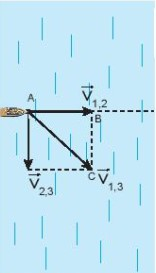
\includegraphics[scale=1]{../figs/VN10-2022-PH-TP005-4.jpg}
	\end{center}
	Gọi vận tốc của ca nô đối với mặt nước là $\vec v_{1,2}$; 
	
	Vận tốc của nước chảy đối với bờ sông là $\vec v_{2,3}$. 
	
	Vận tốc của ca nô đối với bờ sông:
	
	$$\vec v_{1,3} = \vec v_{1,2} + \vec v_{2,3}.$$
	
	Suy ra:
	
	$$v_{1,3} = \sqrt{ v_{1,2}^2 + v_{2,3}^2} = \SI{7,07}{m/s}.$$
	
	Vì $\text{AB} = \text{BC}$ nên tam giác ABC là tam giác vuông cân và góc A bằng $45^\circ$. Hướng của vận tốc nghiêng $45^\circ$ theo hướng Đông - Nam.
}
\item \mkstar{3}


{
	Một máy bay đang bay theo hướng Bắc với vận tốc $\SI{200}{m/s}$ thì bị gió từ hướng Tây thổi vào với vận tốc $\SI{20}{m/s}$. Xác định vận tốc tổng hợp của máy bay lúc này.
}
\hideall
{
	Gọi:
	
	$\vec v_{1,2}$ là vận tốc của máy bay so với gió.
	
	$\vec v_{2,3}$ là vận tốc của gió so với đường bay.
	
	$\vec v_{1,3}$ là vận tốc của máy bay so với đường bay.
	
	Ta có:
	
	$$\vec v_{1,3} = \vec v_{1,2} + \vec v_{2,3}.$$
	
	Vận tốc tổng hợp của máy bay lúc này là
	
	$$v_{1,3} = \sqrt{v_{1,2}^2 + v^2_{2,3}} = \SI{201}{m/s}.$$
}
\item \mkstar{4}


{
	Trên đoàn tàu đang chạy thẳng với vận tốc trung bình $\SI{36}{km/h}$ so với mặt đường, một hành khách đi về đầu tàu với vận tốc $\SI{1}{m/s}$ so với mặt sàn tàu.
	\begin{center}
		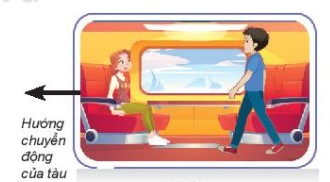
\includegraphics[scale=1]{../figs/VN10-2022-PH-TP005-3.jpg}
	\end{center}
	\begin{enumerate}[label=\alph*)]
		\item Hành khách này tham gia mấy chuyển động?
		\item Làm cách nào để xác định được vận tốc của hành khách đối với mặt đường?
	\end{enumerate}
}
\hideall
{
	\begin{enumerate}[label=\alph*)]
		\item Hành khách này tham gia 2 chuyển động: Chuyển động với vận tốc $\SI{1}{m/s}$ so với sàn tàu và chuyển động do tàu kéo đi với vận tốc bằng vận tốc của tàu so với mặt đường. Chuyển động của hành khách so với mặt đường là tổng hợp của hai chuyển động trên.
		\item Gọi:
		
		- $\vec v_{1,2}$ là vận tốc của hành khách so với tàu.
		
		- $\vec v_{2,3}$ là vận tốc của tàu so với mặt đường.
		
		- $\vec v_{1,3}$ là vận tốc của hành khách so với mặt đường.
		
		Thì:
		
		$$\vec v_{1,3} = \vec v_{1,2} + \vec v_{2,3}$$
		
		Vì các chuyển động trên đều là chuyển động thẳng theo hướng chạy của đoàn tàu nên:
		
		$$v_{1,3} = v_{1,2} + v_{2,3} = \SI{11}{m/s}.$$
		
		Hướng của vận tốc là hướng đoàn tàu chạy.
	\end{enumerate}
}

\item \mkstar{3}


{
	Một người bơi ngang từ bờ bên này sang bờ bên kia của một dòng sông rộng $\SI{50}{m}$ có dòng chảy theo hướng từ Bắc xuống Nam. Do nước sông chảy mạnh nên khi sang đến bờ bên kia thì người đó đã trôi xuôi theo dòng nước $\SI{50}{m}$. Xác định độ dịch chuyển của người đó.
}

\hideall
{
	\begin{center}
		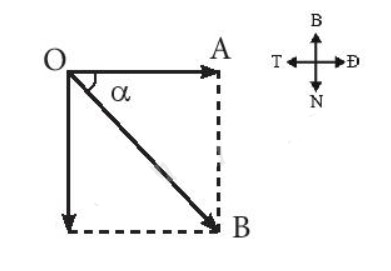
\includegraphics[scale=0.6]{../figs/VN10-2022-PH-TP0001-2.jpg}
	\end{center}
	Người bơi ngang từ bờ bên này sang bên kia theo dự định là OA = $\SI{50}{m}$.
	
	Thực tế, do nước sông chảy mạnh nên vị trí của người đó ở vị trí B, ta có AB = $\SI{50}{m}$.
	
	$\Rightarrow$ Độ dịch chuyển:
	
	$$\Rightarrow\text{OB} = \sqrt{\text{OA}^2 + \text{AB}^2} = \SI{70,7}{km}.$$ 
}
\end{enumerate}